%% latex工作室2021美赛模板,@hope140学习用途以作修改,需要使用xelatex以对中文进行友好支持,由于bib存在,需要进行xe-bib-xe-xe编译,vscode插件可以实现,此编译时间较长

\documentclass{mcmthesis}
\mcmsetup{CTeX = false,   % 使用 CTeX 套装时,设置为 true
        tcn = 0000, problem = A,
        sheet = true, titleinsheet = true, keywordsinsheet = true,
        titlepage = true, abstract = true}

\usepackage[UTF8, scheme = plain]{ctex} % 加入中文支持,注意要在newtxtext之前,以对其他更改保持不变
\usepackage{newtxtext} 

% newtxtext 中对 \@makefnmark 有补丁,使得它对 \thefootnote 会使用专门的上标字体,更美观一些。在 newtxtext 宏包之前定义的 \thefootnote 就会生效;如果在 newtxtext 之后重定义了 \thefootnote,这个功能就取消。
% 在 newtxtext 之后,也可以自己使用 \sustyle 得到对应的上标字体。

% \usepackage{palatino} % 英语艺术字体



\usepackage{lipsum} % 随机生成文本用来测试,正式编辑可以删除

\title{The \LaTeX{} Template for MCM Version \MCMversion}
\author{\small \href{https://www.latexstudio.net/}
  {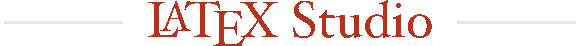
\includegraphics[width=7cm]{mcmthesis-logo}}}
\date{\today}
\begin{document}
\begin{abstract}
Use this template to begin typing the first page (summary page) of your electronic report. This template uses a 12-point Times New Roman font. Submit your paper as an Adobe PDF electronic file (e.g. 1111111.pdf), typed in English, with a readable font of at least 12-point type.

Do not include the name of your school, advisor, or team members on this or any page.

Papers must be within the 25 page limit.

Be sure to change the control number and problem choice above.
You may delete these instructions as you begin to type your report here.

Follow us @COMAPMath on Twitter or COMAPCHINAOFFICIAL on Weibo for the most up to date contest information.

\begin{keywords}
keyword1; keyword2
\end{keywords}
\end{abstract}
\maketitle
%% Generate the Table of Contents, if it's needed.
%% \tableofcontents
%% \newpage
%%
%% Generate the Memorandum, if it's needed.
%% \memoto{\LaTeX{}studio}
%% \memofrom{Liam Huang}
%% \memosubject{Happy \TeX{}ing!}
%% \memodate{\today}
%% \logo{\LARGE I'm pretending to be a LOGO!}
%% \begin{memo}[Memorandum]
%%   \lipsum[1-3]
%% \end{memo}
%%
\section{Introduction}
\subsection{What's this all about? What's \LaTeX?}
\LaTeX\ is a document preparation system which uses the \TeX\
typesetting program. It enables you to produce
publication-quality documents with great accuracy and
consistency. \LaTeX\ works on any computer and produces
industry-standard PDF. It is available both in free (open-source)
and commercial implementations. \LaTeX\ can be used for any kind
of document, but it is especially suited to those with complex
structures, repetitive formatting, or notations like
mathematics. Install the software from
\url{www.tug.org/texlive/}.\cite{邓聚龙1987灰色系统基本方法}
\subsection{Creating and typesetting your document}

\subsection{Syntax (how to type \LaTeX\ commands --- these
  are the rules)}

\lipsum[3]
\begin{itemize}
\item the angular velocity of the bat,
\item the velocity of the ball, and
\item the position of impact along the bat.
\end{itemize}
\lipsum[4]
\emph{center of percussion} [Brody 1986], \lipsum[5]

\begin{Theorem} \label{thm:latex}
\LaTeX
\end{Theorem}
\begin{Lemma} \label{thm:tex}
\TeX .
\end{Lemma}
\begin{proof}
The proof of theorem.
\end{proof}

\subsection{Other Assumptions}
\lipsum[6]
\begin{itemize}
\item
\item
\item
\item
\end{itemize}

\lipsum[7]

\section{Analysis of the Problem}
\begin{figure}[h]
\small
\centering
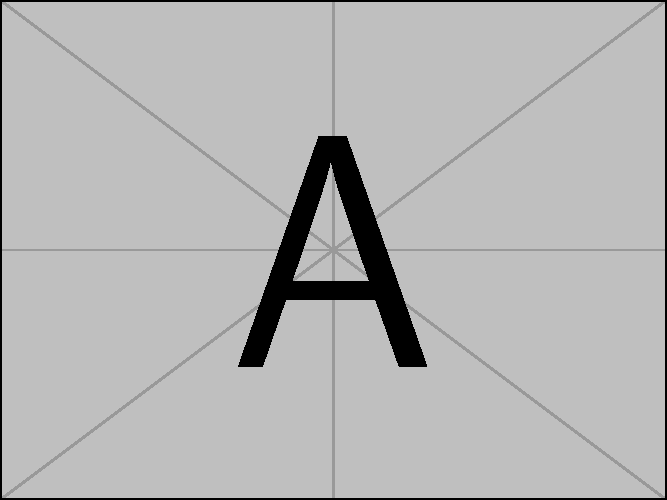
\includegraphics[width=8cm]{example-image-a}
\caption{The name of figure} \label{fig:aa}
\end{figure}

\lipsum[8] \eqref{aa}
\begin{equation}
a^2 \label{aa}
\end{equation}

\[
  \begin{pmatrix}{*{20}c}
  {a_{11} } & {a_{12} } & {a_{13} }  \\
  {a_{21} } & {a_{22} } & {a_{23} }  \\
  {a_{31} } & {a_{32} } & {a_{33} }  \\
  \end{pmatrix}
  = \frac{{Opposite}}{{Hypotenuse}}\cos ^{ - 1} \theta \arcsin \theta
\]
\lipsum[9]

\[
  p_{j}=\begin{cases} 0,&\text{if $j$ is odd}\\
  r!\,(-1)^{j/2},&\text{if $j$ is even}
  \end{cases}
\]

\lipsum[10]

\[
  \arcsin \theta  =
  \mathop{{\int\!\!\!\!\!\int\!\!\!\!\!\int}\mkern-31.2mu
  \bigodot}\limits_\varphi
  {\mathop {\lim }\limits_{x \to \infty } \frac{{n!}}{{r!\left( {n - r}
  \right)!}}} \eqno (1)
\]

\section{Calculating and Simplifying the Model  }
\lipsum[11]

\section{The Model Results}
\lipsum[6]

\section{Validating the Model}
\lipsum[9]

\section{Conclusions}
\lipsum[6]

\section{A Summary}
\lipsum[6]

\section{Evaluate of the Mode}

\section{Strengths and weaknesses}
\lipsum[12]

\subsection{Strengths}
\begin{itemize}
\item \textbf{Applies widely}\\
This  system can be used for many types of airplanes, and it also
solves the interference during  the procedure of the boarding
airplane,as described above we can get to the  optimization
boarding time.We also know that all the service is automate.
\item \textbf{Improve the quality of the airport service}\\
Balancing the cost of the cost and the benefit, it will bring in
more convenient  for airport and passengers.It also saves many
human resources for the airline. \item \textbf{}
\end{itemize}

% 参考文献,这里采用bib “plain”为格式,“mcmthesis-demo”为文件名,由于tex文件第一次编译生成bbl文件名与tex相同,所以这里建议bib使用与tex相同的文件名

\bibliographystyle{plain}

\bibliography{mcmthesis-demo}


%\begin{thebibliography}{99}
%\bibitem{1} D.~E. KNUTH   The \TeX{}book  the American
%Mathematical Society and Addison-Wesley
%Publishing Company , 1984-1986.
%\bibitem{2}Lamport, Leslie,  \LaTeX{}: `` A Document Preparation System '',
%Addison-Wesley Publishing Company, 1986.
%\bibitem{3}\url{https://www.latexstudio.net/}
%\end{thebibliography}

\begin{appendices}

\section{First appendix}

In addition, your report must include a letter to the Chief Financial Officer (CFO) of the Goodgrant Foundation, Mr. Alpha Chiang, that describes the optimal investment strategy, your modeling approach and major results, and a brief discussion of your proposed concept of a return-on-investment (ROI). This letter should be no more than two pages in length.

\begin{letter}{Dear, Mr. Alpha Chiang}

\lipsum[1-2]

\vspace{\parskip}

Sincerely yours,

Your friends

\end{letter}
Here are simulation programmes we used in our model as follow.\\

\textbf{\textcolor[rgb]{0.98,0.00,0.00}{Input matlab source:}}
\lstinputlisting[language=Matlab]{./code/mcmthesis-matlab1.m}

\section{Second appendix}

some more text \textcolor[rgb]{0.98,0.00,0.00}{\textbf{Input C++ source:}}
\lstinputlisting[language=C++]{./code/mcmthesis-sudoku.cpp}

\end{appendices}
\end{document}
%% 
%% This work consists of these files mcmthesis.dtx,
%%                                   figures/ and
%%                                   code/,
%% and the derived files             mcmthesis.cls,
%%                                   mcmthesis-demo.tex,
%%                                   README,
%%                                   LICENSE,
%%                                   mcmthesis.pdf and
%%                                   mcmthesis-demo.pdf.
%%
%% End of file `mcmthesis-demo.tex'.
